\documentclass[10pt,ignorenonframetext,]{beamer}
\setbeamertemplate{caption}[numbered]
\setbeamertemplate{caption label separator}{: }
\setbeamercolor{caption name}{fg=normal text.fg}
\beamertemplatenavigationsymbolsempty
\usepackage{lmodern}
\usepackage{amssymb,amsmath}
\usepackage{ifxetex,ifluatex}
\usepackage{fixltx2e} % provides \textsubscript
\ifnum 0\ifxetex 1\fi\ifluatex 1\fi=0 % if pdftex
  \usepackage[T1]{fontenc}
  \usepackage[utf8]{inputenc}
\else % if luatex or xelatex
  \ifxetex
    \usepackage{mathspec}
  \else
    \usepackage{fontspec}
  \fi
  \defaultfontfeatures{Ligatures=TeX,Scale=MatchLowercase}
\fi
\usetheme[]{Dresden}
\usecolortheme{dolphin}
\usefonttheme{structuresmallcapsserif}
% use upquote if available, for straight quotes in verbatim environments
\IfFileExists{upquote.sty}{\usepackage{upquote}}{}
% use microtype if available
\IfFileExists{microtype.sty}{%
\usepackage{microtype}
\UseMicrotypeSet[protrusion]{basicmath} % disable protrusion for tt fonts
}{}
\newif\ifbibliography
\hypersetup{
            pdftitle={Random Forests},
            pdfauthor={Jan-Philipp Kolb},
            pdfborder={0 0 0},
            breaklinks=true}
\urlstyle{same}  % don't use monospace font for urls
\usepackage{color}
\usepackage{fancyvrb}
\newcommand{\VerbBar}{|}
\newcommand{\VERB}{\Verb[commandchars=\\\{\}]}
\DefineVerbatimEnvironment{Highlighting}{Verbatim}{commandchars=\\\{\}}
% Add ',fontsize=\small' for more characters per line
\newenvironment{Shaded}{}{}
\newcommand{\KeywordTok}[1]{\textcolor[rgb]{0.00,0.00,1.00}{#1}}
\newcommand{\DataTypeTok}[1]{#1}
\newcommand{\DecValTok}[1]{#1}
\newcommand{\BaseNTok}[1]{#1}
\newcommand{\FloatTok}[1]{#1}
\newcommand{\ConstantTok}[1]{#1}
\newcommand{\CharTok}[1]{\textcolor[rgb]{0.00,0.50,0.50}{#1}}
\newcommand{\SpecialCharTok}[1]{\textcolor[rgb]{0.00,0.50,0.50}{#1}}
\newcommand{\StringTok}[1]{\textcolor[rgb]{0.00,0.50,0.50}{#1}}
\newcommand{\VerbatimStringTok}[1]{\textcolor[rgb]{0.00,0.50,0.50}{#1}}
\newcommand{\SpecialStringTok}[1]{\textcolor[rgb]{0.00,0.50,0.50}{#1}}
\newcommand{\ImportTok}[1]{#1}
\newcommand{\CommentTok}[1]{\textcolor[rgb]{0.00,0.50,0.00}{#1}}
\newcommand{\DocumentationTok}[1]{\textcolor[rgb]{0.00,0.50,0.00}{#1}}
\newcommand{\AnnotationTok}[1]{\textcolor[rgb]{0.00,0.50,0.00}{#1}}
\newcommand{\CommentVarTok}[1]{\textcolor[rgb]{0.00,0.50,0.00}{#1}}
\newcommand{\OtherTok}[1]{\textcolor[rgb]{1.00,0.25,0.00}{#1}}
\newcommand{\FunctionTok}[1]{#1}
\newcommand{\VariableTok}[1]{#1}
\newcommand{\ControlFlowTok}[1]{\textcolor[rgb]{0.00,0.00,1.00}{#1}}
\newcommand{\OperatorTok}[1]{#1}
\newcommand{\BuiltInTok}[1]{#1}
\newcommand{\ExtensionTok}[1]{#1}
\newcommand{\PreprocessorTok}[1]{\textcolor[rgb]{1.00,0.25,0.00}{#1}}
\newcommand{\AttributeTok}[1]{#1}
\newcommand{\RegionMarkerTok}[1]{#1}
\newcommand{\InformationTok}[1]{\textcolor[rgb]{0.00,0.50,0.00}{#1}}
\newcommand{\WarningTok}[1]{\textcolor[rgb]{0.00,0.50,0.00}{\textbf{#1}}}
\newcommand{\AlertTok}[1]{\textcolor[rgb]{1.00,0.00,0.00}{#1}}
\newcommand{\ErrorTok}[1]{\textcolor[rgb]{1.00,0.00,0.00}{\textbf{#1}}}
\newcommand{\NormalTok}[1]{#1}
\usepackage{graphicx,grffile}
\makeatletter
\def\maxwidth{\ifdim\Gin@nat@width>\linewidth\linewidth\else\Gin@nat@width\fi}
\def\maxheight{\ifdim\Gin@nat@height>\textheight0.8\textheight\else\Gin@nat@height\fi}
\makeatother
% Scale images if necessary, so that they will not overflow the page
% margins by default, and it is still possible to overwrite the defaults
% using explicit options in \includegraphics[width, height, ...]{}
\setkeys{Gin}{width=\maxwidth,height=\maxheight,keepaspectratio}

% Prevent slide breaks in the middle of a paragraph:
\widowpenalties 1 10000
\raggedbottom

\AtBeginPart{
  \let\insertpartnumber\relax
  \let\partname\relax
  \frame{\partpage}
}
\AtBeginSection{
  \ifbibliography
  \else
    \let\insertsectionnumber\relax
    \let\sectionname\relax
    \frame{\sectionpage}
  \fi
}
\AtBeginSubsection{
  \let\insertsubsectionnumber\relax
  \let\subsectionname\relax
  \frame{\subsectionpage}
}

\setlength{\parindent}{0pt}
\setlength{\parskip}{6pt plus 2pt minus 1pt}
\setlength{\emergencystretch}{3em}  % prevent overfull lines
\providecommand{\tightlist}{%
  \setlength{\itemsep}{0pt}\setlength{\parskip}{0pt}}
\setcounter{secnumdepth}{0}

\title{Random Forests}
\author{Jan-Philipp Kolb}
\date{20 Mai, 2019}

\begin{document}
\frame{\titlepage}

\begin{frame}{Random Forests}

\begin{itemize}
\tightlist
\item
  Bagging (bootstrap aggregating) regression trees is a technique that
  can turn a single tree model with high variance and poor predictive
  power into a fairly accurate prediction function.
\item
  Unfortunately, bagging regression trees typically suffers from tree
  correlation, which reduces the overall performance of the model.
\item
  Random forests are a modification of bagging that builds a large
  collection of de-correlated trees and have become a very popular
  ``out-of-the-box'' learning algorithm that enjoys good predictive
  performance.
\end{itemize}

\end{frame}

\begin{frame}[fragile]{Preparation - random forests}

\begin{itemize}
\tightlist
\item
  The following slides are based on UC Business Analytics R Programming
  Guide on \href{http://uc-r.github.io/random_forests}{random forests}
\end{itemize}

\begin{Shaded}
\begin{Highlighting}[]
\KeywordTok{library}\NormalTok{(rsample)      }\CommentTok{# data splitting }
\KeywordTok{library}\NormalTok{(randomForest) }\CommentTok{# basic implementation}
\KeywordTok{library}\NormalTok{(ranger)       }\CommentTok{# a faster implementation of randomForest}
\KeywordTok{library}\NormalTok{(caret)        }\CommentTok{# an aggregator package for performing many machine learning models}
\KeywordTok{library}\NormalTok{(h2o)          }\CommentTok{# an extremely fast java-based platform}
\end{Highlighting}
\end{Shaded}

\end{frame}

\begin{frame}[fragile]{The Ames housing data}

\begin{Shaded}
\begin{Highlighting}[]
\KeywordTok{set.seed}\NormalTok{(}\DecValTok{123}\NormalTok{)}
\NormalTok{ames_split <-}\StringTok{ }\KeywordTok{initial_split}\NormalTok{(AmesHousing}\OperatorTok{::}\KeywordTok{make_ames}\NormalTok{(), }\DataTypeTok{prop =}\NormalTok{ .}\DecValTok{7}\NormalTok{)}
\NormalTok{ames_train <-}\StringTok{ }\KeywordTok{training}\NormalTok{(ames_split)}
\NormalTok{ames_test  <-}\StringTok{ }\KeywordTok{testing}\NormalTok{(ames_split)}
\end{Highlighting}
\end{Shaded}

\end{frame}

\begin{frame}{The idea of random forests}

\begin{itemize}
\tightlist
\item
  Random forests are built on the same fundamental principles as
  decision trees and bagging.
\item
  Bagging trees introduces a random component in to the tree building
  process that reduces the variance of a single tree's prediction and
  improves predictive performance.
\item
  The trees in bagging are not completely independent of each other
  since all the original predictors are considered at every split of
  every tree.
\item
  Trees from different bootstrap samples typically have similar
  structure to each other (especially at the top of the tree) due to
  underlying relationships.
\end{itemize}

\end{frame}

\begin{frame}[fragile]{Similar trees}

\begin{itemize}
\tightlist
\item
  E.g., if we create six decision trees with different bootstrapped
  samples of the Boston housing data, we see that the top of the trees
  all have a very similar structure.
\item
  Although there are 15 predictor variables to split on, all six trees
  have both \texttt{lstat} and \texttt{rm} variables driving the first
  few splits.
\end{itemize}

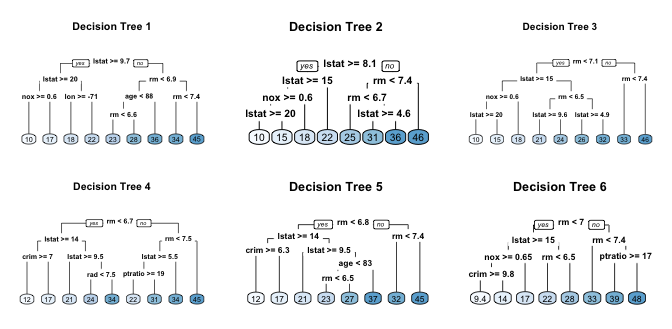
\includegraphics{figure/tree-correlation-1.png}

\end{frame}

\begin{frame}{Tree correlation}

\begin{itemize}
\tightlist
\item
  This characteristic is known as tree correlation and prevents bagging
  from optimally reducing variance of the predictive values.
\item
  In order to reduce variance further, we need to minimize the amount of
  correlation between the trees.
\item
  This can be achieved by injecting more randomness into the
  tree-growing process. Random forests achieve this in two ways:
\end{itemize}

\begin{block}{1. Bootstrap:}

\begin{itemize}
\tightlist
\item
  Similar to bagging, each tree is grown to a bootstrap resampled data
  set, which makes them different and somewhat decorrelates them.
\end{itemize}

\end{block}

\begin{block}{2. Split-variable randomization:}

\begin{itemize}
\tightlist
\item
  Each time a split is to be performed, the search for the split
  variable is limited to a random subset of m of the p variables.
\item
  For regression trees, typical default values are \(m=\dfrac{p}{3}\)
  but this should be considered a tuning parameter.
\item
  When \(m=p\), the randomization amounts to using only step 1 and is
  the same as bagging.
\end{itemize}

\end{block}

\end{frame}

\begin{frame}[fragile]{Basic algorithm}

The basic algorithm for a regression random forest can be generalized to
the following:

\begin{verbatim}
1.  Given training data set
2.  Select number of trees to build (ntrees)
3.  for i = 1 to ntrees do
4.  |  Generate a bootstrap sample of the original data
5.  |  Grow a regression tree to the bootstrapped data
6.  |  for each split do
7.  |  | Select m variables at random from all p variables
8.  |  | Pick the best variable/split-point among the m
9.  |  | Split the node into two child nodes
10. |  end
11. | Use typical tree model stopping criteria to determine when a tree is complete (but do not prune)
12. end
\end{verbatim}

\begin{itemize}
\tightlist
\item
  Since the algorithm randomly selects a bootstrap sample to train on
  and predictors to use at each split, tree correlation will be lessened
  beyond bagged trees.
\end{itemize}

\end{frame}

\begin{frame}{OOB error vs.~test set error}

\begin{itemize}
\tightlist
\item
  Similar to bagging, a natural benefit of the bootstrap resampling
  process is that random forests have an out-of-bag (OOB) sample that
  provides an efficient and reasonable approximation of the test error.
\item
  This provides a built-in validation set without any extra work on your
  part, and you do not need to sacrifice any of your training data to
  use for validation.
\item
  This makes identifying the number of trees required to stablize the
  error rate during tuning more efficient;
\item
  As illustrated below some difference between the OOB error and test
  error are expected.
\end{itemize}

\end{frame}

\begin{frame}{Random forest out-of-bag error versus validation error}

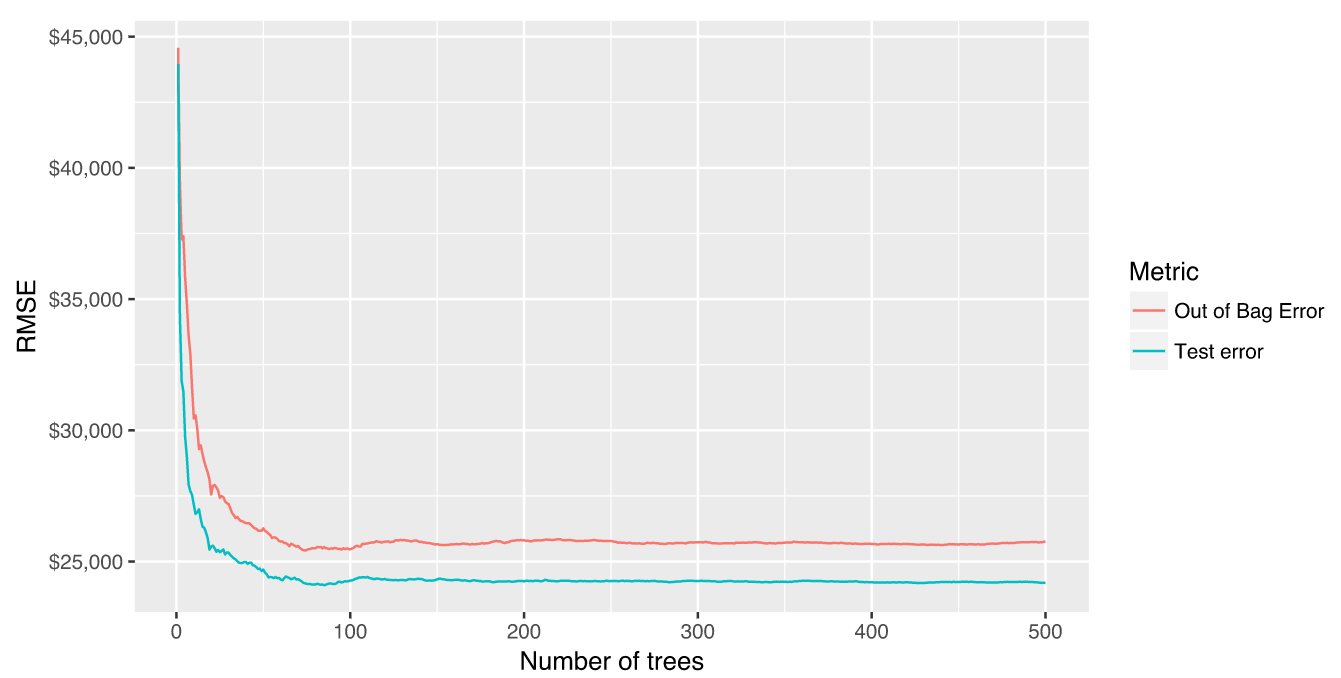
\includegraphics{figure/random_trees_fig1.PNG}

\end{frame}

\begin{frame}{Scoring models - metrics}

\begin{itemize}
\tightlist
\item
  Many packages do not keep track of which observations were part of the
  OOB sample for a given tree and which were not.
\item
  If you are comparing multiple models to one-another, you'd want to
  score each on the same validation set to compare performance.
\item
  It is possible to compute certain metrics such as root mean squared
  logarithmic error (RMSLE) on the OOB sample, but it is not built in to
  all packages.
\item
  So if you are looking to compare multiple models or use a slightly
  less traditional loss function you will likely want to still perform
  cross validation.
\end{itemize}

\end{frame}

\begin{frame}{Advantages \& Disadvantages}

\begin{block}{Advantages - random forrests}

\begin{itemize}
\tightlist
\item
  Typically have very good performance
\item
  Remarkably good ``out-of-the box'' - very little tuning required
\item
  Built-in validation set - don't need to sacrifice data for extra
  validation
\item
  No pre-processing required
\item
  Robust to outliers
\end{itemize}

\end{block}

\begin{block}{Disadvantages - random forrests}

\begin{itemize}
\tightlist
\item
  Can become slow on large data sets
\item
  Although accurate, often cannot compete with advanced boosting
  algorithms
\item
  Less interpretable
\end{itemize}

\end{block}

\end{frame}

\begin{frame}[fragile]{Basic implementation}

\begin{itemize}
\tightlist
\item
  There are over 20 random forest packages in R.
\item
  To demonstrate the basic implementation we illustrate the use of the
  \texttt{randomForest} package, the oldest and most well known
  implementation of the Random Forest algorithm in R.
\item
  As your data set grows in size \texttt{randomForest} does not scale
  well (although you can parallelize with \texttt{foreach}).
\item
  To explore and compare a variety of tuning parameters we can also find
  more effective packages.
\item
  The packages \texttt{ranger} and \texttt{h2o} packages will be
  presented in the tuning section.
\end{itemize}

\end{frame}

\begin{frame}[fragile]{\texttt{randomForest::randomForest}}

\begin{itemize}
\tightlist
\item
  \texttt{randomForest} can use the formula or separate x, y matrix
  notation for specifying our model.
\item
  Below we apply the default \texttt{randomForest} model using the
  formulaic specification.
\item
  The default random forest performs 500 trees and
  \(\dfrac{\text{features}}{3}=26\) randomly selected predictor
  variables at each split.
\item
  Averaging across all 500 trees provides an OOB MSE=659550782
  (RMSE=25682).
\end{itemize}

\begin{Shaded}
\begin{Highlighting}[]
\KeywordTok{set.seed}\NormalTok{(}\DecValTok{123}\NormalTok{)}
\CommentTok{# default RF model}
\NormalTok{m1 <-}\StringTok{ }\KeywordTok{randomForest}\NormalTok{(}\DataTypeTok{formula =}\NormalTok{ Sale_Price }\OperatorTok{~}\StringTok{ }\NormalTok{.,}\DataTypeTok{data=}\NormalTok{ames_train)}
\NormalTok{m1}
\end{Highlighting}
\end{Shaded}

\begin{verbatim}
## 
## Call:
##  randomForest(formula = Sale_Price ~ ., data = ames_train) 
##                Type of random forest: regression
##                      Number of trees: 500
## No. of variables tried at each split: 26
## 
##           Mean of squared residuals: 661089658
##                     % Var explained: 89.8
\end{verbatim}

\end{frame}

\begin{frame}[fragile]{Plotting the model}

\begin{itemize}
\tightlist
\item
  Plotting the model will illustrate the error rate as we average across
  more trees and shows that our error rate stabalizes with around 100
  trees but continues to decrease slowly until around 300 or so trees.
\end{itemize}

\begin{Shaded}
\begin{Highlighting}[]
\KeywordTok{plot}\NormalTok{(m1)}
\end{Highlighting}
\end{Shaded}

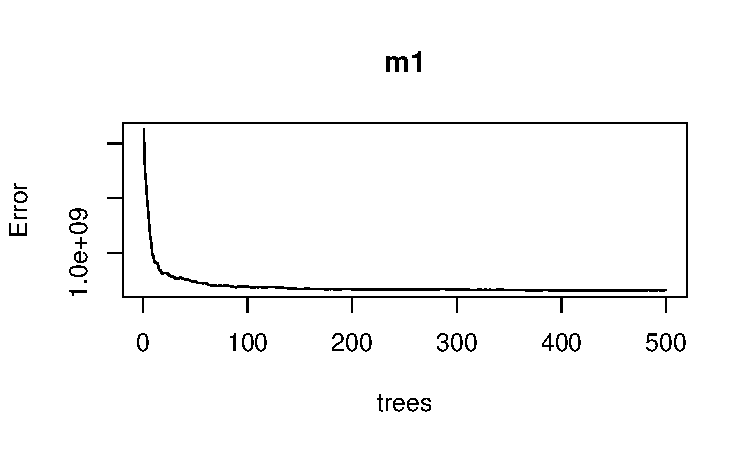
\includegraphics{c2_random_forests_files/figure-beamer/unnamed-chunk-5-1.pdf}

\end{frame}

\begin{frame}[fragile]{The plotted error rate}

\begin{itemize}
\tightlist
\item
  The plotted error rate above is based on the OOB sample error and can
  be accessed directly at \texttt{m1\$mse}.
\item
  We can find which number of trees providing the lowest error rate,
  which is 344 trees providing an average home sales price error of
  \$25,673.
\end{itemize}

\begin{Shaded}
\begin{Highlighting}[]
\KeywordTok{which.min}\NormalTok{(m1}\OperatorTok{$}\NormalTok{mse)}
\end{Highlighting}
\end{Shaded}

\begin{verbatim}
## [1] 447
\end{verbatim}

\begin{Shaded}
\begin{Highlighting}[]
\KeywordTok{sqrt}\NormalTok{(m1}\OperatorTok{$}\NormalTok{mse[}\KeywordTok{which.min}\NormalTok{(m1}\OperatorTok{$}\NormalTok{mse)])}
\end{Highlighting}
\end{Shaded}

\begin{verbatim}
## [1] 25648.78
\end{verbatim}

\end{frame}

\begin{frame}[fragile]{A validation set to measure predictive accuracy}

\begin{itemize}
\tightlist
\item
  \texttt{randomForest} also allows us to use a validation set to
  measure predictive accuracy if we did not want to use the OOB samples.
\item
  Here we split our training set further to create a training and
  validation set.
\item
  We then supply the validation data in the \texttt{xtest} and
  \texttt{ytest} arguments.
\end{itemize}

\begin{Shaded}
\begin{Highlighting}[]
\KeywordTok{set.seed}\NormalTok{(}\DecValTok{123}\NormalTok{)}
\NormalTok{valid_split <-}\StringTok{ }\KeywordTok{initial_split}\NormalTok{(ames_train, .}\DecValTok{8}\NormalTok{)}
\CommentTok{# training data}
\NormalTok{ames_train_v2 <-}\StringTok{ }\KeywordTok{analysis}\NormalTok{(valid_split)}
\CommentTok{# validation data}
\NormalTok{ames_valid <-}\StringTok{ }\KeywordTok{assessment}\NormalTok{(valid_split)}
\NormalTok{x_test <-}\StringTok{ }\NormalTok{ames_valid[}\KeywordTok{setdiff}\NormalTok{(}\KeywordTok{names}\NormalTok{(ames_valid), }\StringTok{"Sale_Price"}\NormalTok{)]}
\NormalTok{y_test <-}\StringTok{ }\NormalTok{ames_valid}\OperatorTok{$}\NormalTok{Sale_Price}
\end{Highlighting}
\end{Shaded}

\end{frame}

\begin{frame}[fragile]{Extract OOB \& validation errors}

\begin{Shaded}
\begin{Highlighting}[]
\NormalTok{rf_oob_comp <-}\StringTok{ }\KeywordTok{randomForest}\NormalTok{(}\DataTypeTok{formula=}\NormalTok{Sale_Price }\OperatorTok{~}\StringTok{ }\NormalTok{.,}
  \DataTypeTok{data=}\NormalTok{ames_train_v2,}\DataTypeTok{xtest =}\NormalTok{ x_test,}\DataTypeTok{ytest=}\NormalTok{y_test)}
\NormalTok{oob <-}\StringTok{ }\KeywordTok{sqrt}\NormalTok{(rf_oob_comp}\OperatorTok{$}\NormalTok{mse) }\CommentTok{# extract OOB & validation errors}
\NormalTok{validation <-}\StringTok{ }\KeywordTok{sqrt}\NormalTok{(rf_oob_comp}\OperatorTok{$}\NormalTok{test}\OperatorTok{$}\NormalTok{mse)}
\end{Highlighting}
\end{Shaded}

\begin{Shaded}
\begin{Highlighting}[]
\CommentTok{# compare error rates}
\NormalTok{tibble}\OperatorTok{::}\KeywordTok{tibble}\NormalTok{(}
  \StringTok{`}\DataTypeTok{Out of Bag Error}\StringTok{`}\NormalTok{ =}\StringTok{ }\NormalTok{oob,}
  \StringTok{`}\DataTypeTok{Test error}\StringTok{`}\NormalTok{ =}\StringTok{ }\NormalTok{validation,}
  \DataTypeTok{ntrees =} \DecValTok{1}\OperatorTok{:}\NormalTok{rf_oob_comp}\OperatorTok{$}\NormalTok{ntree}
\NormalTok{) }\OperatorTok
\StringTok{  }\KeywordTok{gather}\NormalTok{(Metric, RMSE, }\OperatorTok{-}\NormalTok{ntrees) }\OperatorTok
\StringTok{  }\KeywordTok{ggplot}\NormalTok{(}\KeywordTok{aes}\NormalTok{(ntrees, RMSE, }\DataTypeTok{color =}\NormalTok{ Metric)) }\OperatorTok{+}
\StringTok{  }\KeywordTok{geom_line}\NormalTok{() }\OperatorTok{+}
\StringTok{  }\KeywordTok{scale_y_continuous}\NormalTok{(}\DataTypeTok{labels =}\NormalTok{ scales}\OperatorTok{::}\NormalTok{dollar) }\OperatorTok{+}
\StringTok{  }\KeywordTok{xlab}\NormalTok{(}\StringTok{"Number of trees"}\NormalTok{)}
\end{Highlighting}
\end{Shaded}

\end{frame}

\begin{frame}{Compare error rates}

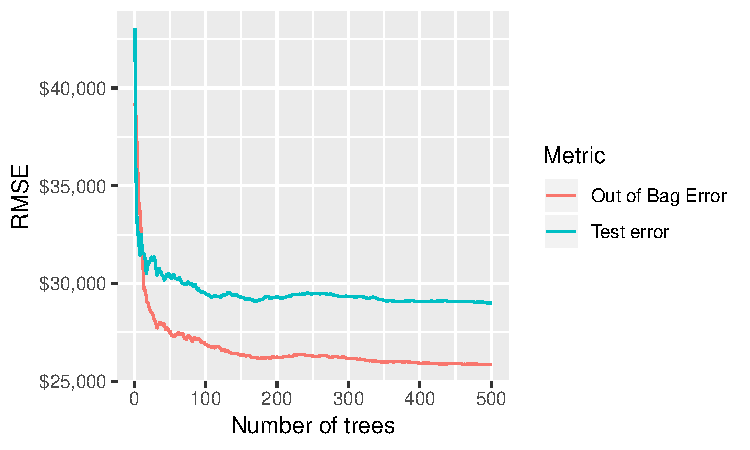
\includegraphics{c2_random_forests_files/figure-beamer/unnamed-chunk-10-1.pdf}

\end{frame}

\begin{frame}{Random forests - out-of-the-box algorithm}

\begin{itemize}
\tightlist
\item
  Random forests are one of the best ``out-of-the-box'' machine learning
  algorithms.
\item
  They typically perform remarkably well with very little tuning
  required. - - E.g., we were able to get an RMSE of less than 30K
  Dollar without any tuning which is over a 6K Dollar reduction to the
  RMSE achieved with a fully-tuned bagging model and \$4K reduction to
  to a fully-tuned elastic net model.
\item
  We can still seek improvement by tuning our random forest model.
\end{itemize}

\end{frame}

\begin{frame}{Tuning}

\begin{itemize}
\tightlist
\item
  Random forests are fairly easy to tune since there are only a handful
  of tuning parameters.
\item
  Typically, the primary concern at the beginning is tuning the number
  of candidate variables to select from at each split.
\item
  There are a few additional hyperparameters that we should be aware of.
\item
  The argument names may differ across packages, but these
  hyperparameters should be present:
\end{itemize}

\end{frame}

\begin{frame}[fragile]{Tuning parameters}

\begin{itemize}
\tightlist
\item
  \texttt{ntree}: number of trees. We want enough trees to stabalize the
  error but using too many trees is unncessarily inefficient, especially
  when using large data sets.
\item
  \texttt{mtry}: the number of variables to randomly sample as
  candidates at each split. When \texttt{mtry} =p the model equates to
  bagging. When \texttt{mtry=1} the split variable is completely random,
  so all variables get a chance but can lead to overly biased results. A
  common suggestion is to start with 5 values evenly spaced across the
  range from 2 to p.
\item
  \texttt{sampsize}: the number of samples to train on. The default
  value is 63.25\% of the training set since this is the expected value
  of unique observations in the bootstrap sample. Lower sample sizes can
  reduce the training time but may introduce more bias than necessary.
  Increasing the sample size can increase performance but at the risk of
  overfitting because it introduces more variance. Typically, when
  tuning this parameter we stay near the 60-80\% range.
\item
  \texttt{nodesize}: minimum number of samples within the terminal
  nodes. Controls the complexity of the trees. Smaller node size allows
  for deeper, more complex trees and smaller node results in shallower
  trees. This is another bias-variance tradeoff where deeper trees
  introduce more variance (risk of overfitting) and shallower trees
  introduce more bias (risk of not fully capturing unique patters and
  relatonships in the data).
\item
  \texttt{maxnodes}: maximum number of terminal nodes. Another way to
  control the complexity of the trees. More nodes equates to deeper,
  more complex trees and less nodes result in shallower trees.
\end{itemize}

\end{frame}

\begin{frame}[fragile]{Initial tuning with \texttt{randomForest}}

\begin{itemize}
\tightlist
\item
  If we are interested with just starting out and tuning the mtry
  parameter we can use \texttt{randomForest::tuneRF} for a quick and
  easy tuning assessment.
\item
  \texttt{tuneRf} will start at a value of mtry that you supply and
  increase by a certain step factor until the OOB error stops improving
  be a specified amount.
\item
  For example, the below starts with mtry = 5 and increases by a factor
  of 1.5 until the OOB error stops improving by 1 per cent.
\item
  Note that \texttt{tuneRF} requires a separate x y specification.
\item
  We see that the optimal \texttt{mtry} value in this sequence is very
  close to the default mtry value of \(\dfrac{\text{features}{3}=26\).
\end{itemize}

\end{frame}

\begin{frame}[fragile]{Names of features}

\begin{Shaded}
\begin{Highlighting}[]
\NormalTok{features <-}\StringTok{ }\KeywordTok{setdiff}\NormalTok{(}\KeywordTok{names}\NormalTok{(ames_train), }\StringTok{"Sale_Price"}\NormalTok{)}

\KeywordTok{set.seed}\NormalTok{(}\DecValTok{123}\NormalTok{)}

\NormalTok{m2 <-}\StringTok{ }\KeywordTok{tuneRF}\NormalTok{(}
  \DataTypeTok{x          =}\NormalTok{ ames_train[features],}
  \DataTypeTok{y          =}\NormalTok{ ames_train}\OperatorTok{$}\NormalTok{Sale_Price,}
  \DataTypeTok{ntreeTry   =} \DecValTok{500}\NormalTok{,}
  \DataTypeTok{mtryStart  =} \DecValTok{5}\NormalTok{,}
  \DataTypeTok{stepFactor =} \FloatTok{1.5}\NormalTok{,}
  \DataTypeTok{improve    =} \FloatTok{0.01}\NormalTok{,}
  \DataTypeTok{trace      =} \OtherTok{FALSE}      \CommentTok{# to not show real-time progress }
\NormalTok{)}
\end{Highlighting}
\end{Shaded}

\begin{verbatim}
## -0.06304958 0.01 
## 0.05261869 0.01 
## 0.03755382 0.01 
## 0.04358806 0.01 
## 0.01959577 0.01 
## -0.01941831 0.01
\end{verbatim}

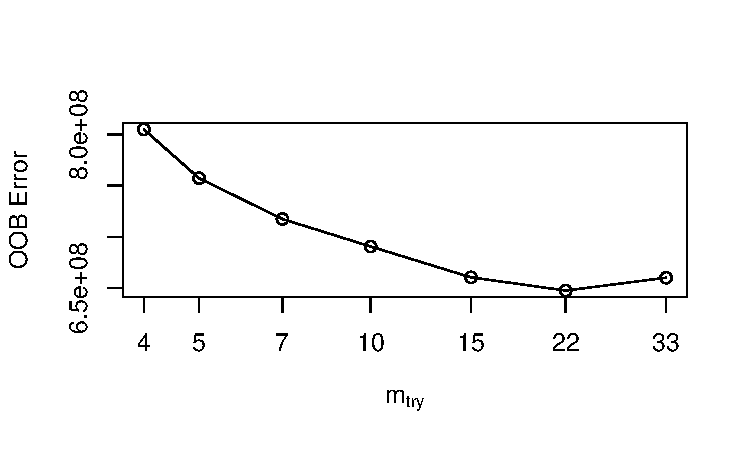
\includegraphics{c2_random_forests_files/figure-beamer/unnamed-chunk-11-1.pdf}

\end{frame}

\begin{frame}[fragile]{Full grid search with \texttt{ranger}}

\begin{itemize}
\tightlist
\item
  To perform a larger grid search across several hyperparameters we'll
  need to create a grid and loop through each hyperparameter combination
  and evaluate the model.
\item
  Unfortunately, this is where \texttt{randomForest} becomes quite
  inefficient since it does not scale well.
\item
  Instead, we can use \texttt{ranger} which is a C++ implementation of
  Brieman's random forest algorithm and, as the following illustrates,
  is over 6 times faster than \texttt{randomForest}.
\end{itemize}

\end{frame}

\begin{frame}[fragile]{Assessing the speed}

\begin{block}{\texttt{randomForest} speed}

\begin{Shaded}
\begin{Highlighting}[]
\KeywordTok{system.time}\NormalTok{(}
\NormalTok{  ames_randomForest <-}\StringTok{ }\KeywordTok{randomForest}\NormalTok{(}
    \DataTypeTok{formula =}\NormalTok{ Sale_Price }\OperatorTok{~}\StringTok{ }\NormalTok{., }
    \DataTypeTok{data    =}\NormalTok{ ames_train, }
    \DataTypeTok{ntree   =} \DecValTok{500}\NormalTok{,}
    \DataTypeTok{mtry    =} \KeywordTok{floor}\NormalTok{(}\KeywordTok{length}\NormalTok{(features) }\OperatorTok{/}\StringTok{ }\DecValTok{3}\NormalTok{)}
\NormalTok{  )}
\NormalTok{)}
\end{Highlighting}
\end{Shaded}

\begin{verbatim}
##    user  system elapsed 
##   45.66    0.09   45.88
\end{verbatim}

\end{block}

\begin{block}{ranger speed}

\begin{Shaded}
\begin{Highlighting}[]
\KeywordTok{system.time}\NormalTok{(}
\NormalTok{  ames_ranger <-}\StringTok{ }\KeywordTok{ranger}\NormalTok{(}
    \DataTypeTok{formula   =}\NormalTok{ Sale_Price }\OperatorTok{~}\StringTok{ }\NormalTok{., }
    \DataTypeTok{data      =}\NormalTok{ ames_train, }
    \DataTypeTok{num.trees =} \DecValTok{500}\NormalTok{,}
    \DataTypeTok{mtry      =} \KeywordTok{floor}\NormalTok{(}\KeywordTok{length}\NormalTok{(features) }\OperatorTok{/}\StringTok{ }\DecValTok{3}\NormalTok{)}
\NormalTok{  )}
\NormalTok{)}
\end{Highlighting}
\end{Shaded}

\begin{verbatim}
##    user  system elapsed 
##    4.73    0.00    1.41
\end{verbatim}

\end{block}

\end{frame}

\begin{frame}[fragile]{The grid search}

\begin{itemize}
\tightlist
\item
  To perform the grid search, first we want to construct our grid of
  hyperparameters.
\item
  We're going to search across 96 different models with varying
  \texttt{mtry}, minimum node size, and sample size.
\end{itemize}

\begin{Shaded}
\begin{Highlighting}[]
\CommentTok{# hyperparameter grid search}
\NormalTok{hyper_grid <-}\StringTok{ }\KeywordTok{expand.grid}\NormalTok{(}
  \DataTypeTok{mtry       =} \KeywordTok{seq}\NormalTok{(}\DecValTok{20}\NormalTok{, }\DecValTok{30}\NormalTok{, }\DataTypeTok{by =} \DecValTok{2}\NormalTok{),}
  \DataTypeTok{node_size  =} \KeywordTok{seq}\NormalTok{(}\DecValTok{3}\NormalTok{, }\DecValTok{9}\NormalTok{, }\DataTypeTok{by =} \DecValTok{2}\NormalTok{),}
  \DataTypeTok{sampe_size =} \KeywordTok{c}\NormalTok{(.}\DecValTok{55}\NormalTok{, .}\DecValTok{632}\NormalTok{, .}\DecValTok{70}\NormalTok{, .}\DecValTok{80}\NormalTok{),}
  \DataTypeTok{OOB_RMSE   =} \DecValTok{0}
\NormalTok{)}

\KeywordTok{nrow}\NormalTok{(hyper_grid) }\CommentTok{# total number of combinations}
\end{Highlighting}
\end{Shaded}

\begin{verbatim}
## [1] 96
\end{verbatim}

\end{frame}

\begin{frame}{}

\begin{itemize}
\tightlist
\item
  We loop through each hyperparameter combination and apply 500 trees
  since our previous examples illustrated that 500 was plenty to achieve
  a stable error rate.
\item
  We set the random number generator seed. This allows us to
  consistently sample the same observations for each sample size and
  make it more clear the impact that each change makes.
\item
  Our OOB RMSE ranges between \(\tilde\) 26,000-27,000.
\item
  Our top 10 performing models all have RMSE values right around 26,000
  and the results show that models with slighly larger sample sizes
  (70-80\%) and deeper trees (3-5 observations in an terminal node)
  perform best.
\item
  We get a full range of mtry values showing up in our top 10 so is does
  not look like that is over influential.
\end{itemize}

\end{frame}

\end{document}
